The brain uses information from multiple sensory modalities to construct a flexible representation of the body, including its current structure and position (Dijkerman and de Haan, 2007; Makin et al., 2008; Tsakiris, 2010; Blanke, 2012; Ehrsson, 2012). For such a body representation, vision and proprioception continually provide estimates of (changing) limb position, which is crucial to guide actions (Wolpert et al., 1998; Graziano and Botvinick, 2002; Holmes and Spence, 2004). Behavioral experiments using prisms or mirrors have shown that visuo-proprioceptive limb position information is integrated based on the relative reliability of the unisensory modalities, with vision usually “dominating” proprioception due to its higher spatial acuity (van Beers et al., 1999; Holmes and Spence, 2005). This is also suggested by the rubber hand illusion (RHI) (Botvinick and Cohen, 1998), in which visual position information from a fake hand “overrides” proprioception after visuo-tactile costimulation of the fake hand and the real hand. Notably, the RHI only works if the fake hand is in a position similar to the real hand (Pavani et al., 2000; Ehrsson et al., 2004; Lloyd, 2007; Makin et al., 2008), which implies that the brain only integrates visuo-proprioceptive information under sufficient cross-modal congruence.
https://www.jneurosci.org/content/36/9/2582 















We then wanted to investigate further into effect of discrepancy between vision and proprioception. We expect that when vision and proprioception are congruent, the accuracy if highest, because of the formation of target location representation with respect to the hand. Conversely, when vision and proprioception are incongruent, we hypothesize different outcomes depending on the weight attributed by the system to each sensory modality. \cite{fossataro2020immersive} If system relies more on proprioception, the effect of visual hand distance from the target will not be significant, suggesting that the coding of target space is centered on real hand. If system relies more on vision, there will be a significant effect of VH-T distance, suggesting the shift of coding of multi-sensory space on visual hand. REFER to FOSSATARO2020 FOR MORE.
\section{Reporting LME results}

We first used a series of linear mixed-effects models to test whether participants’ judgments of the possibility of the five different kinds of events differed across time pressure/delay conditions (SI Text, Statistical Approach). We observed an effect of whether participants were reflectively deliberating, χ2(1)=20.653
, P<0.001
, and an effect of event-type χ2(4)=860.48
, P<0.001
. Critically, however, these main effects were qualified by a deliberation ×
 event-type interaction, χ2(4)=64.093
, P<0.001
. We decomposed this interaction, using a series of generalized linear models.

\section{Ancillary results from Experiment1}

Also, for all 12 conditions, subject-wise Variability in reach error was calculated, by computing the standard deviation of bias of a particular subject for a particular condition.

For reach error variability, the two-way ANOVA showed that a significant main effect of target position was present ( $F(1.34 26.87) = 21.161 , p = 2.36e-05, \eta_{p}^{2} = 0.514$ ). The main effect of Non-Action Hand Information, and the interaction effect between the two factors were not significant. Post-hoc pairwise comparisons for analysing the differences in reach error variability due to target positions, using the paired t-test, showed significant differences between the Left and the Center target positions ($p = 1.10e-04$), between the Left and Right target position (1.84e-08), and between the Center and the Right target position ($p = 1.47e-05$). 


\section{Introduction}

One of the most fundamental experiences of a human is interacting with the environment through reaching action. Reaching action underlies diverse capabilities of human life, including feeding oneself and object manipulation. \cite{kim_psychology_2021} One of the characteristics of reaching action is that it is directed at external objects of interests, that is, reaching action is characteristically goal-directed. These objects of interest serve as targets for the agent to make contact with. To perform a successful reach, the cognitive system of the agent requires knowledge regarding not just the targets of the action, but also regarding the state of the effector, the entity with which the action is performed. For example, if an agent intends to make contact with the coffee mug, they require knowledge of the spatial location of their hand and the spatial location of the coffee mug. Thus, a successful reaching action requires perception of the objects the agent is acting on and the state of the effector by which the agent is acting with. \cite{wong2014multimodality}

Vision is one of the perceptual modalities through which knowledge regarding the objects of action is provided. Knowledge regarding the state of the effector is also provided through vision. Furthermore, proprioception is an interoceptive perceptual modality which also provides knowledge regarding the state of the effector, specifically regarding the relative positions of the body parts.
\cite{wong2014multimodality}

Body schema is a term used to describe the representation of the body which is utilized for action planning and action control. Both visual and proprioceptive information is integrated to form body schema.

The question that we are interested in exploring through this research is as follows- How does the body schema play a role in reaching action? We claim that body schema not only provides knowledge regarding the state of the effector, about it also affects the perception of the target object itself. 

To investigate this claim, we induced uncertainty in the state of the effector, that is, the hand by which the reaching action is performed, by rendering the action hand invisible in an immersive virtual reality environment. We then manipulated the visual and the proprioceptive information of a body part which was not directly relevant to the reaching action, that is the hand by which action was not performed. The subjects then performed reaches towards the target, with their action hands rendered invisible. We hypothesized that the accuracy in estimating the spatial location of the reach target would be greater when visuo-proprioceptive information about the non-action hand is present, compared to the condition when the no information is provided about the non-action hand.  

Our results show that subjects are more accurate in estimating the location of the target, when the visuo-proprioceptive information regarding the other hand is present, even though the other hand is not directly irrelevant to the reaching action. The accuracy is not significantly improved if only visual or only proprioceptive information about the non-action hand is present. 

The question that follows is- even though the (non-action) hand is task irrelevant, why does the visuo-proprioceptive information about it affect the way the target location is estimated? The explanation could be that the target is represented with respect to the non-action hand. For this representation to occur, visuo-proprioceptive information about the body needs to be available and integrated with each other, that is, integration of visuo-proprioceptive information may be necessary for egocentric representation of reaching action target. 

    
The computation of estimating target location may be understood as a process of probabilistic inference, in which the subject attempts to infer the most probable location of the target, by utilizing sensory inputs and prior knowledge about the state of the environment. Therefore, we have modelled the target location estimation data as a Bayesian decision model. In a Bayesian decision model, the subject assigns probabilities to all possible contact locations, on the basis of a noisy sensory measurement signal of the target and prior beliefs about which target location is more probable.
    
We are investigating whether the presence and absence of visuo-proprioceptive signals of the body affect the uncertainty in the measurement of the sensory observation. Furthermore, we are also investigating whether the visuo-proprioceptive signals affect the subject's beliefs about the probabilities of different target locations.

%We applied a simple Bayesian Model of Perceptual Inference to behavioral data and assessed how model parameters shift when subjects are aware of priors compared to when priors are implicitly learned under different conditions of Non-action Hand Information.
%NOTES!!!!Firing is highest when there is least visuo-proprioceptive discrepency



The results of the Likelihood Ratio Test for model comparison suggest that the interaction between the visuo-proprioceptive discrepancy and the distance between Proprioceptive Hand and the Target (PHT) is a significant reach error predictor.

Figure \ref{fig:exp2_re-pht} shows the effect of PHT on reach error at different levels of discrepancy. The graph reveals following insights:
\begin{itemize}

\item As the distance between the proprioceptive hand and the target increases, there is lesser effect of different levels of discrepancy on reach error. On the other hand, when the target is closer to the proprioceptive hand, varying reach errors are observed for different levels of visuo-proprioceptive discrepancy. 

\item Let us consider discrepancy = 0 as a baseline condition, where visual and proprioceptive inputs are spatially congruent. In this condition, there is a slight underestimation of the target location towards the action hand. 

\item As the visuo-proprioceptive discrepancy increases, with the visual hand being rendered closer to the target (discrepancy = +5.75cm), the reaches are more accurate. This suggests that the visual hand may be used as an anchor for the target representation due to its proximity to the target despite the discrepancy between the visual and proprioceptive inputs of the hand.

\item However, as the discrepancy increases further, with visual hand moving even closer to the target (discrepancy = 11.5cm), the estimate of the target location is pulled towards the visual hand, as indicated by the negative values of the reach errors. This "pull" effect diminishes as the distance between the target and the proprioceptive hand increases. However, the close proximity of visual hand and target seems to increase the accuracy even though the visuo-proprioceptive discrepancy is high and when the target is far from the proprioceptive hand.

\item In contrast, when the visuo-proprioceptive discrepancy is induced by rendering the visual hand away from the targets (discrepancy = -5.75cm and -11.50cm), overall high values of reach error are observed. The reach error increases with increasing distance between the target and proprioceptive hand, and then decreases. This decrease in reach error may indicate the pull effect due to the influence of proximity to the action action, though the reach error remains higher than in the conditions with zero and positive discrepancy levels. 

\end{itemize}

%\begin{figure}[t]
\centering       
    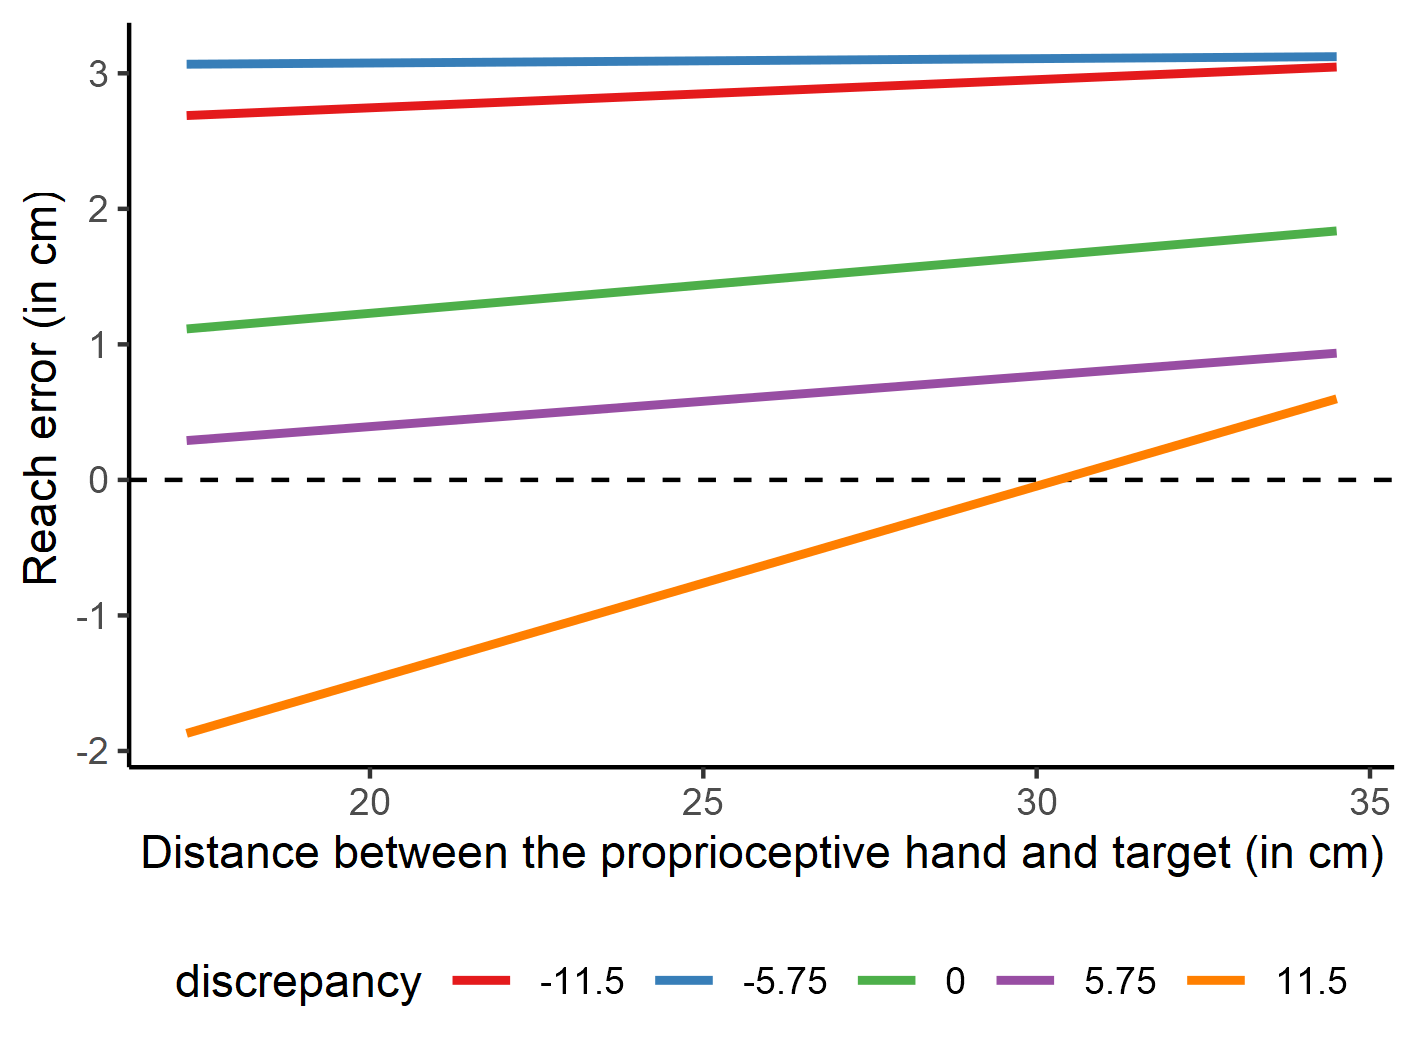
\includegraphics[scale=0.8]{Images/exp2_results.png}
    \caption{Reach error as a function of spatial discrepancy between the position of visual hand and the position of actual (proprioceptive) non-action hand. Each panel shows the distance between the target and the initial position of the action hand (AHT). Negative reach error indicates that the estimation of the target location was in the direction of the non-action hand towards the left, while positive reach error indicates that the location of the target was estimated in the direction of action hand towards the right of the actual location of the target.}
    \label{fig:exp2_re-pht}
\end{figure}
%\begin{figure}[t]
\centering       
    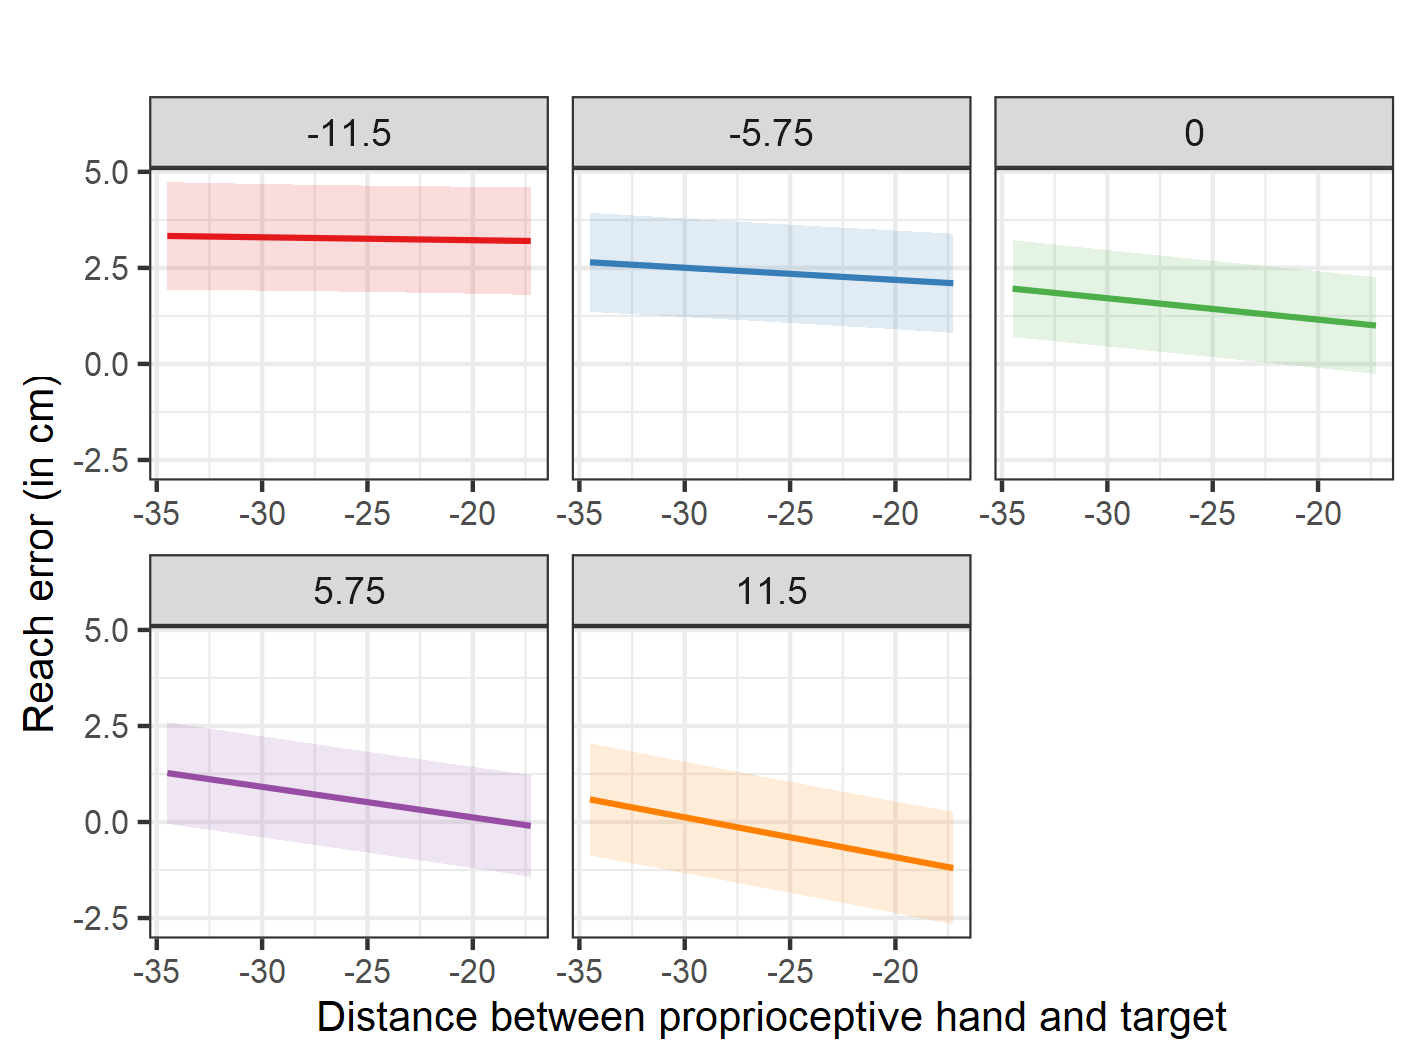
\includegraphics[scale=0.7]{Images/margeff.png}
    \caption{Marginal effect plot}
    \label{fig:exp2-margeff}
\end{figure}

Overall, the results suggest that the target being in the proximity to the visual hand seems to elicit an estimation of the target location which is relatively pulled towards the non-action hand.






